\documentclass{article}
\usepackage[margin=2cm]{geometry}
\usepackage{float}
\usepackage{graphicx}
\usepackage{hyperref}
\usepackage{lscape}
\usepackage{pdflscape}


% Paragraph settings
\setlength{\parskip}{10pt plus 1pt minus 1pt
\setlength{\parindent}{0cm}}

\begin{document}
\title{CS22310 - Hotel Site Assignment}
\author{Samuel Jackson \\ \texttt{slj11@aber.ac.uk}}
\date{\today}
\maketitle

\section{Introduction}
This document provides the final report for the CS22310 Hotel Site assignment and contains the task analysis, interaction design, documentation of prototype and discussion of usability principles. The prototype implementation for this site can be found at \url{http://users.aber.ac.uk/slj11/cs22310/index.html}

\section{Task Analysis}
This section of the document details the analysis of the brief and the identification for the major tasks that the system needs to perform along with characterisation of the users that will perform these tasks. The analysis is documented using a rich picture, use case, data flow and state transition diagrams along with an accompanying description of each.

\subsection{Rich Picture and Identification of Users}
For the first step in my task analysis, I created a rich picture to provide a high level overview of the proposed system and try and identify its major functions and users.

\begin{figure}[H]
\centering
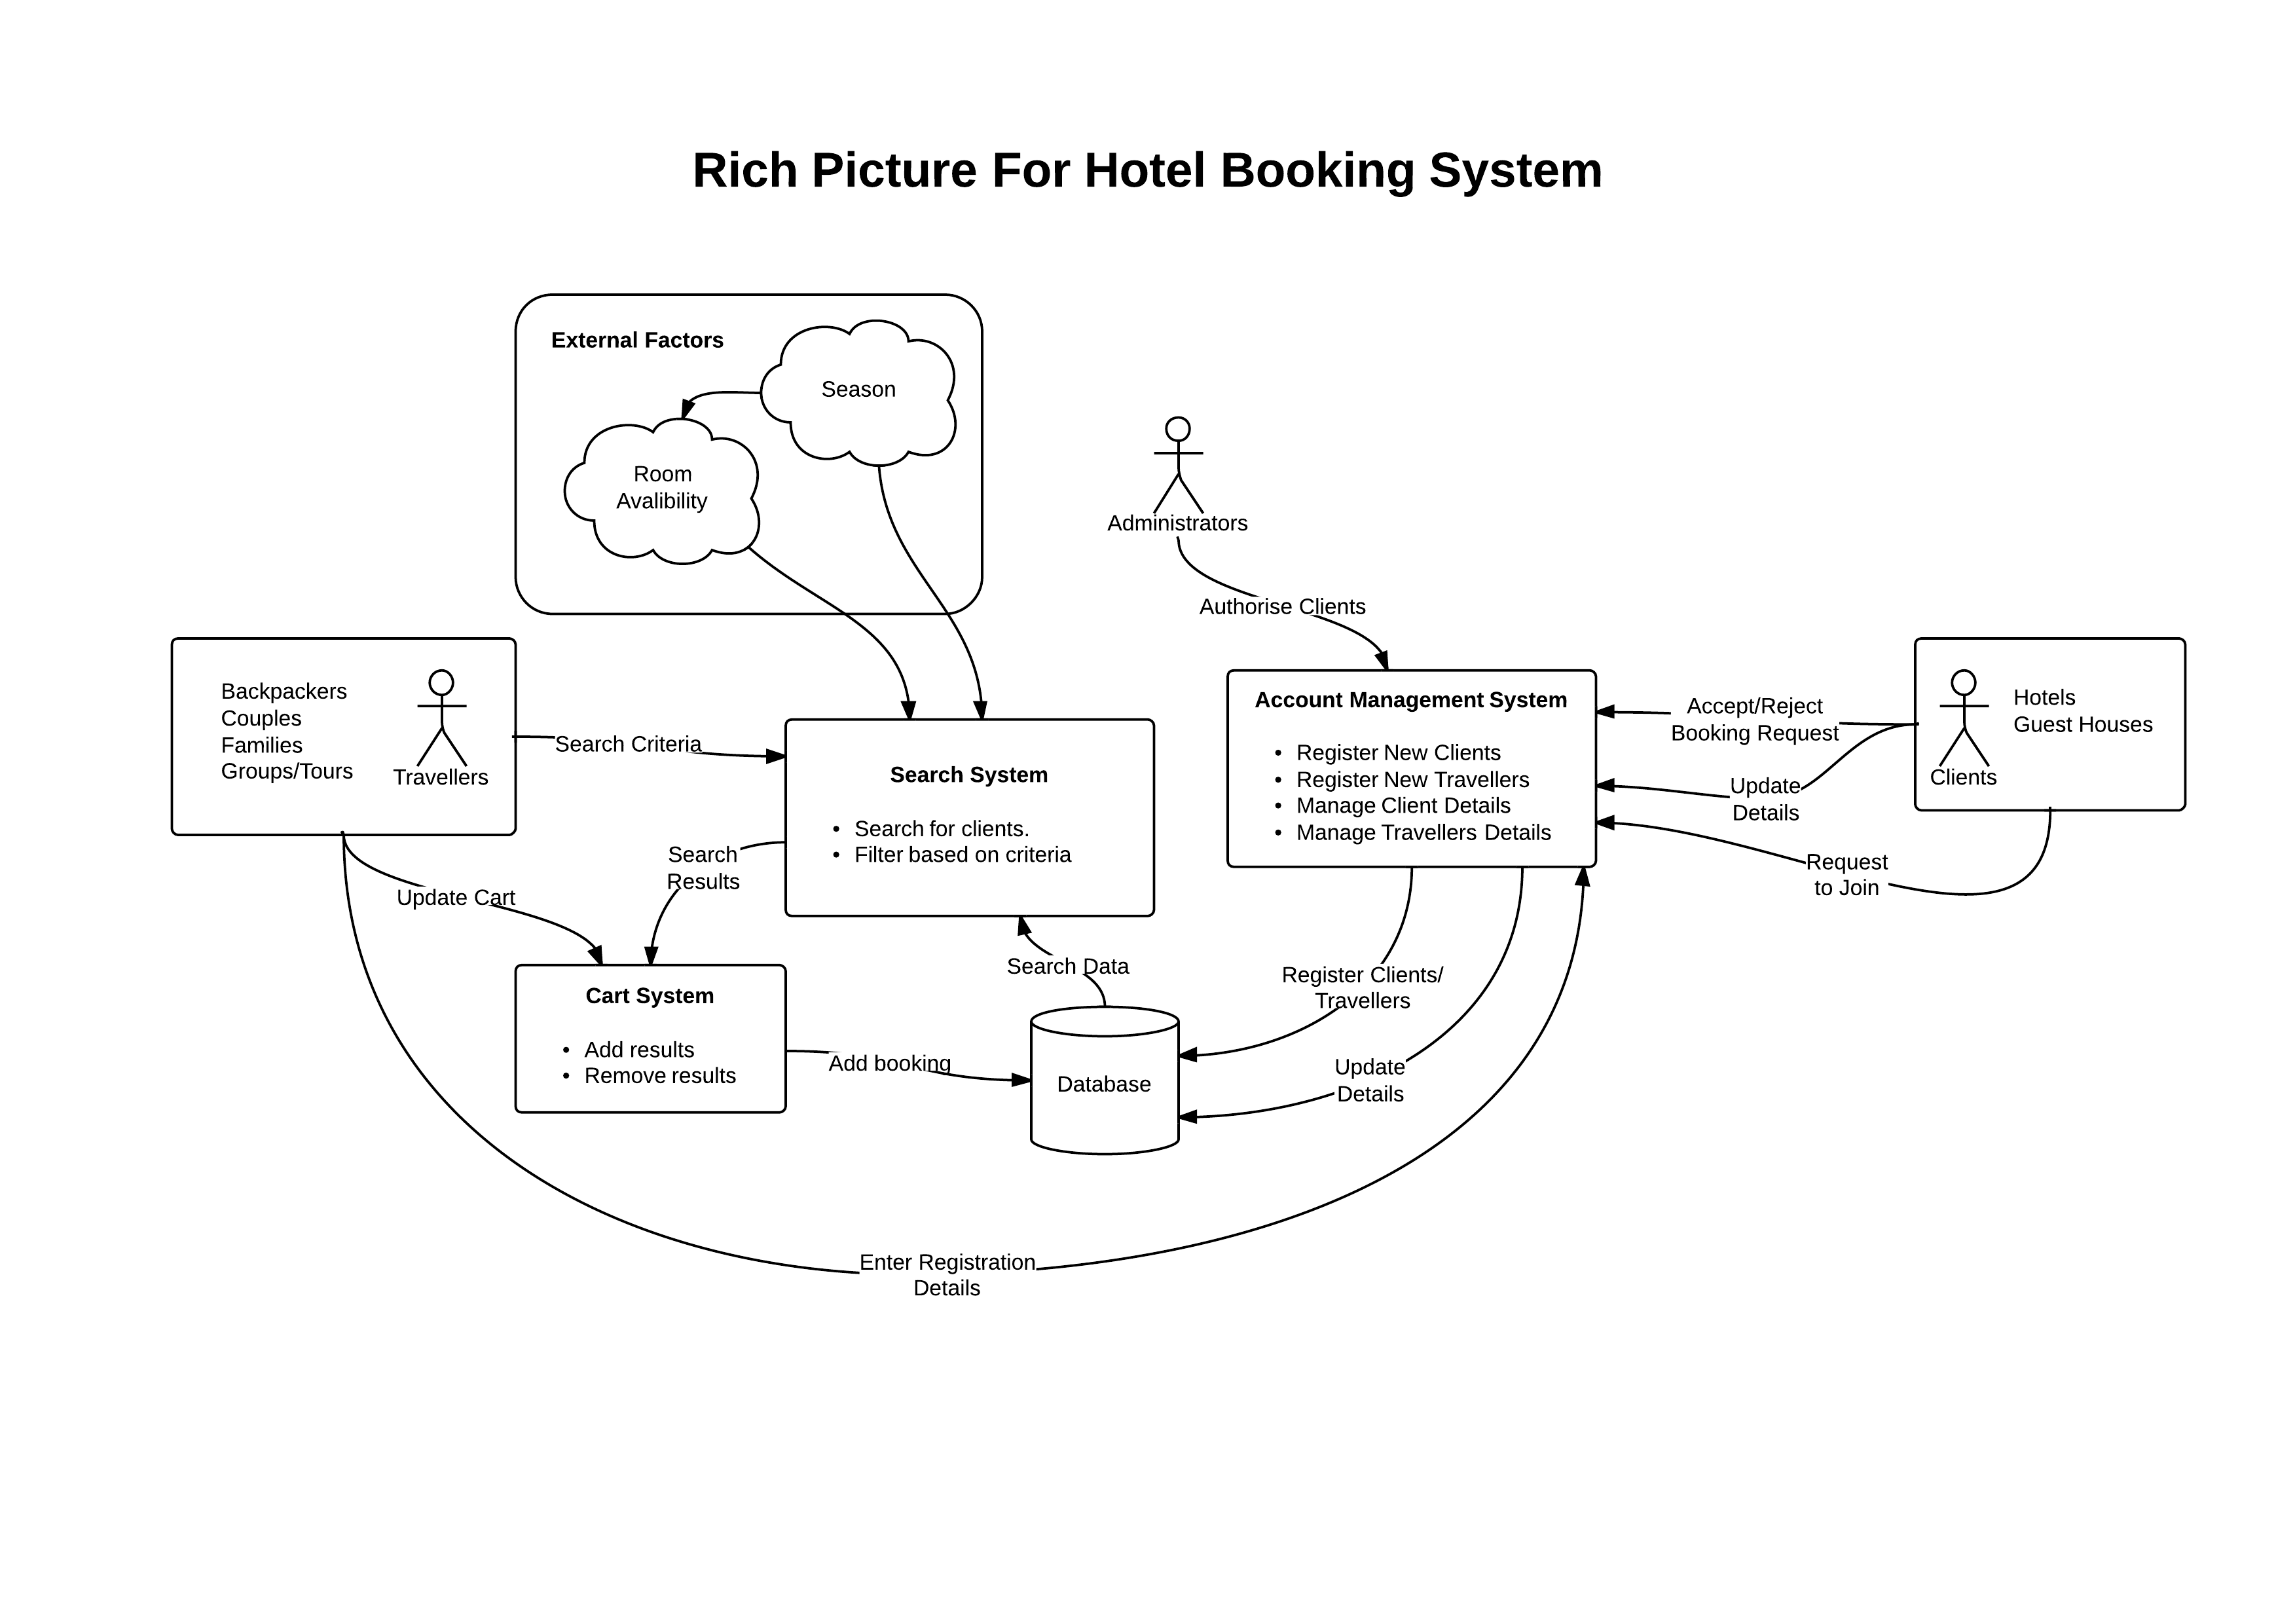
\includegraphics[width=1\textwidth]{img/richpic.png}
\caption{Rich Picture for the Hotel Site}
\label{fig:rich-pic}
\end{figure}

In this diagram, I have identified three key users of the system and three major "task areas" that our system must be able to perform. The major actors in the system are as follows:
\begin{itemize}
	\item \textbf{Travellers} - Travellers are customers of the hotel booking site who wish to search and book lodging with the hotels and guest houses listed on the site.
	\item \textbf{Clients} - Clients are also customers of the hotel booking site, but are representatives or managers of various hotels and guest houses which can register an account with the site to list there available accommodation.
	\item \textbf{Administrators} - Administrators are employees of the hotel booking site and who's only major function is to authorise requests by clients for registration with the site.
\end{itemize}

Of the three major types of users identified here, the most technologically inexperienced are most likely to be the Travellers. This is due to the potentially wide variety of different customers that could use the site as this a diverse user demographic implies a wide diversity in technological competency. They  will also have almost no training in how to use the system (unlike administrators and possibly clients). It is therefore paramount that system functions undertaken by Travellers be as clear and accessible as possible. Travellers may be either single contact (they only use the site once) or may be repeat customers. Therefore there interface should accommodate inexperienced "first time" users while still providing ease of access for power users.

Clients are likely to be similar to travellers, but perhaps with slightly less diversity in competency. This is due to the fact that the hotel/guest house may have a dedicated member of staff (such as a manager) that is responsible for dealing with the management of hotel's listing on the site. This employee may also receive training by an employee which already knows how to use the system. However, when a new client registers with the hotel site, the client management interface stills needs to be intuitive to the first time users. This point is particularly relevant the smaller hotels and guest houses who are more likely to not have a technical professional to handle the establishments web presence.

Client will have a recurring connection with hotel site and there connection is most likely going to last for months and years, rather than being a single one off connection with the site like some potential Travellers. Again it is stressed that this section of the site be accessible to a variety of user skill levels. It is also more of a requirement that this part of the site be efficient. Client users are not looking to "browse" like Travellers but are coming to the site to perform a specific task (e.g. updating promotional information) and therefore want clear and easy to use interface to quick accomplish the task the came to do.

The final major type of system user are administrators. Administrators are likely to be the most technically competent users. They are expected to have frequent, recurrent contact with the system, probably on a daily basis. They are also likely to be well trained by the company running the hotel booking site. Like Clients, they will not wish to "browse" the site, but will come to it in order to carry out a specific task and therefore will want a clear and efficient interface suitable for a power user.

The rich picture also identifies three key categories that user tasks fall into across the site. The first category of task are those related to the management of the accounts associated with users. This includes tasks that allow the Clients to update information about their establishment, the registration of Client and Travellers and Travellers updating their payment and billing information. Task in this category are carried out by each of the types of system users.

In contrast, the other two categories that system tasks fall into are only carried out by Travellers. These two areas are the search system and the cart/payment system. Both of these areas are distinct but closely related. In fact, the search system feeds into the cart and payment system. However, the search system is concerned with getting results that match the users criteria and refining there choices. The cart system is designed to guide the user through the payment and booking process after they have finished making their choices. Note that the picture also displays some external influences on the search system which ma affect the results available to Travellers, such as room availability and the season.

As a final note, I have also added the a data store labelled database. This is the major data sink on the hotel site server where information about bookings, hotel and user accounts all feed into. Data is pulled from this store and displayed via the interface as required.

\subsection{System Tasks}
The next step in task analysis is to analyse, at a high level, the actions that can be performed by each of the identified users within the system. In order to clear identify each of these actions, the following use case diagram is provided.

\begin{figure}[H]
\centering
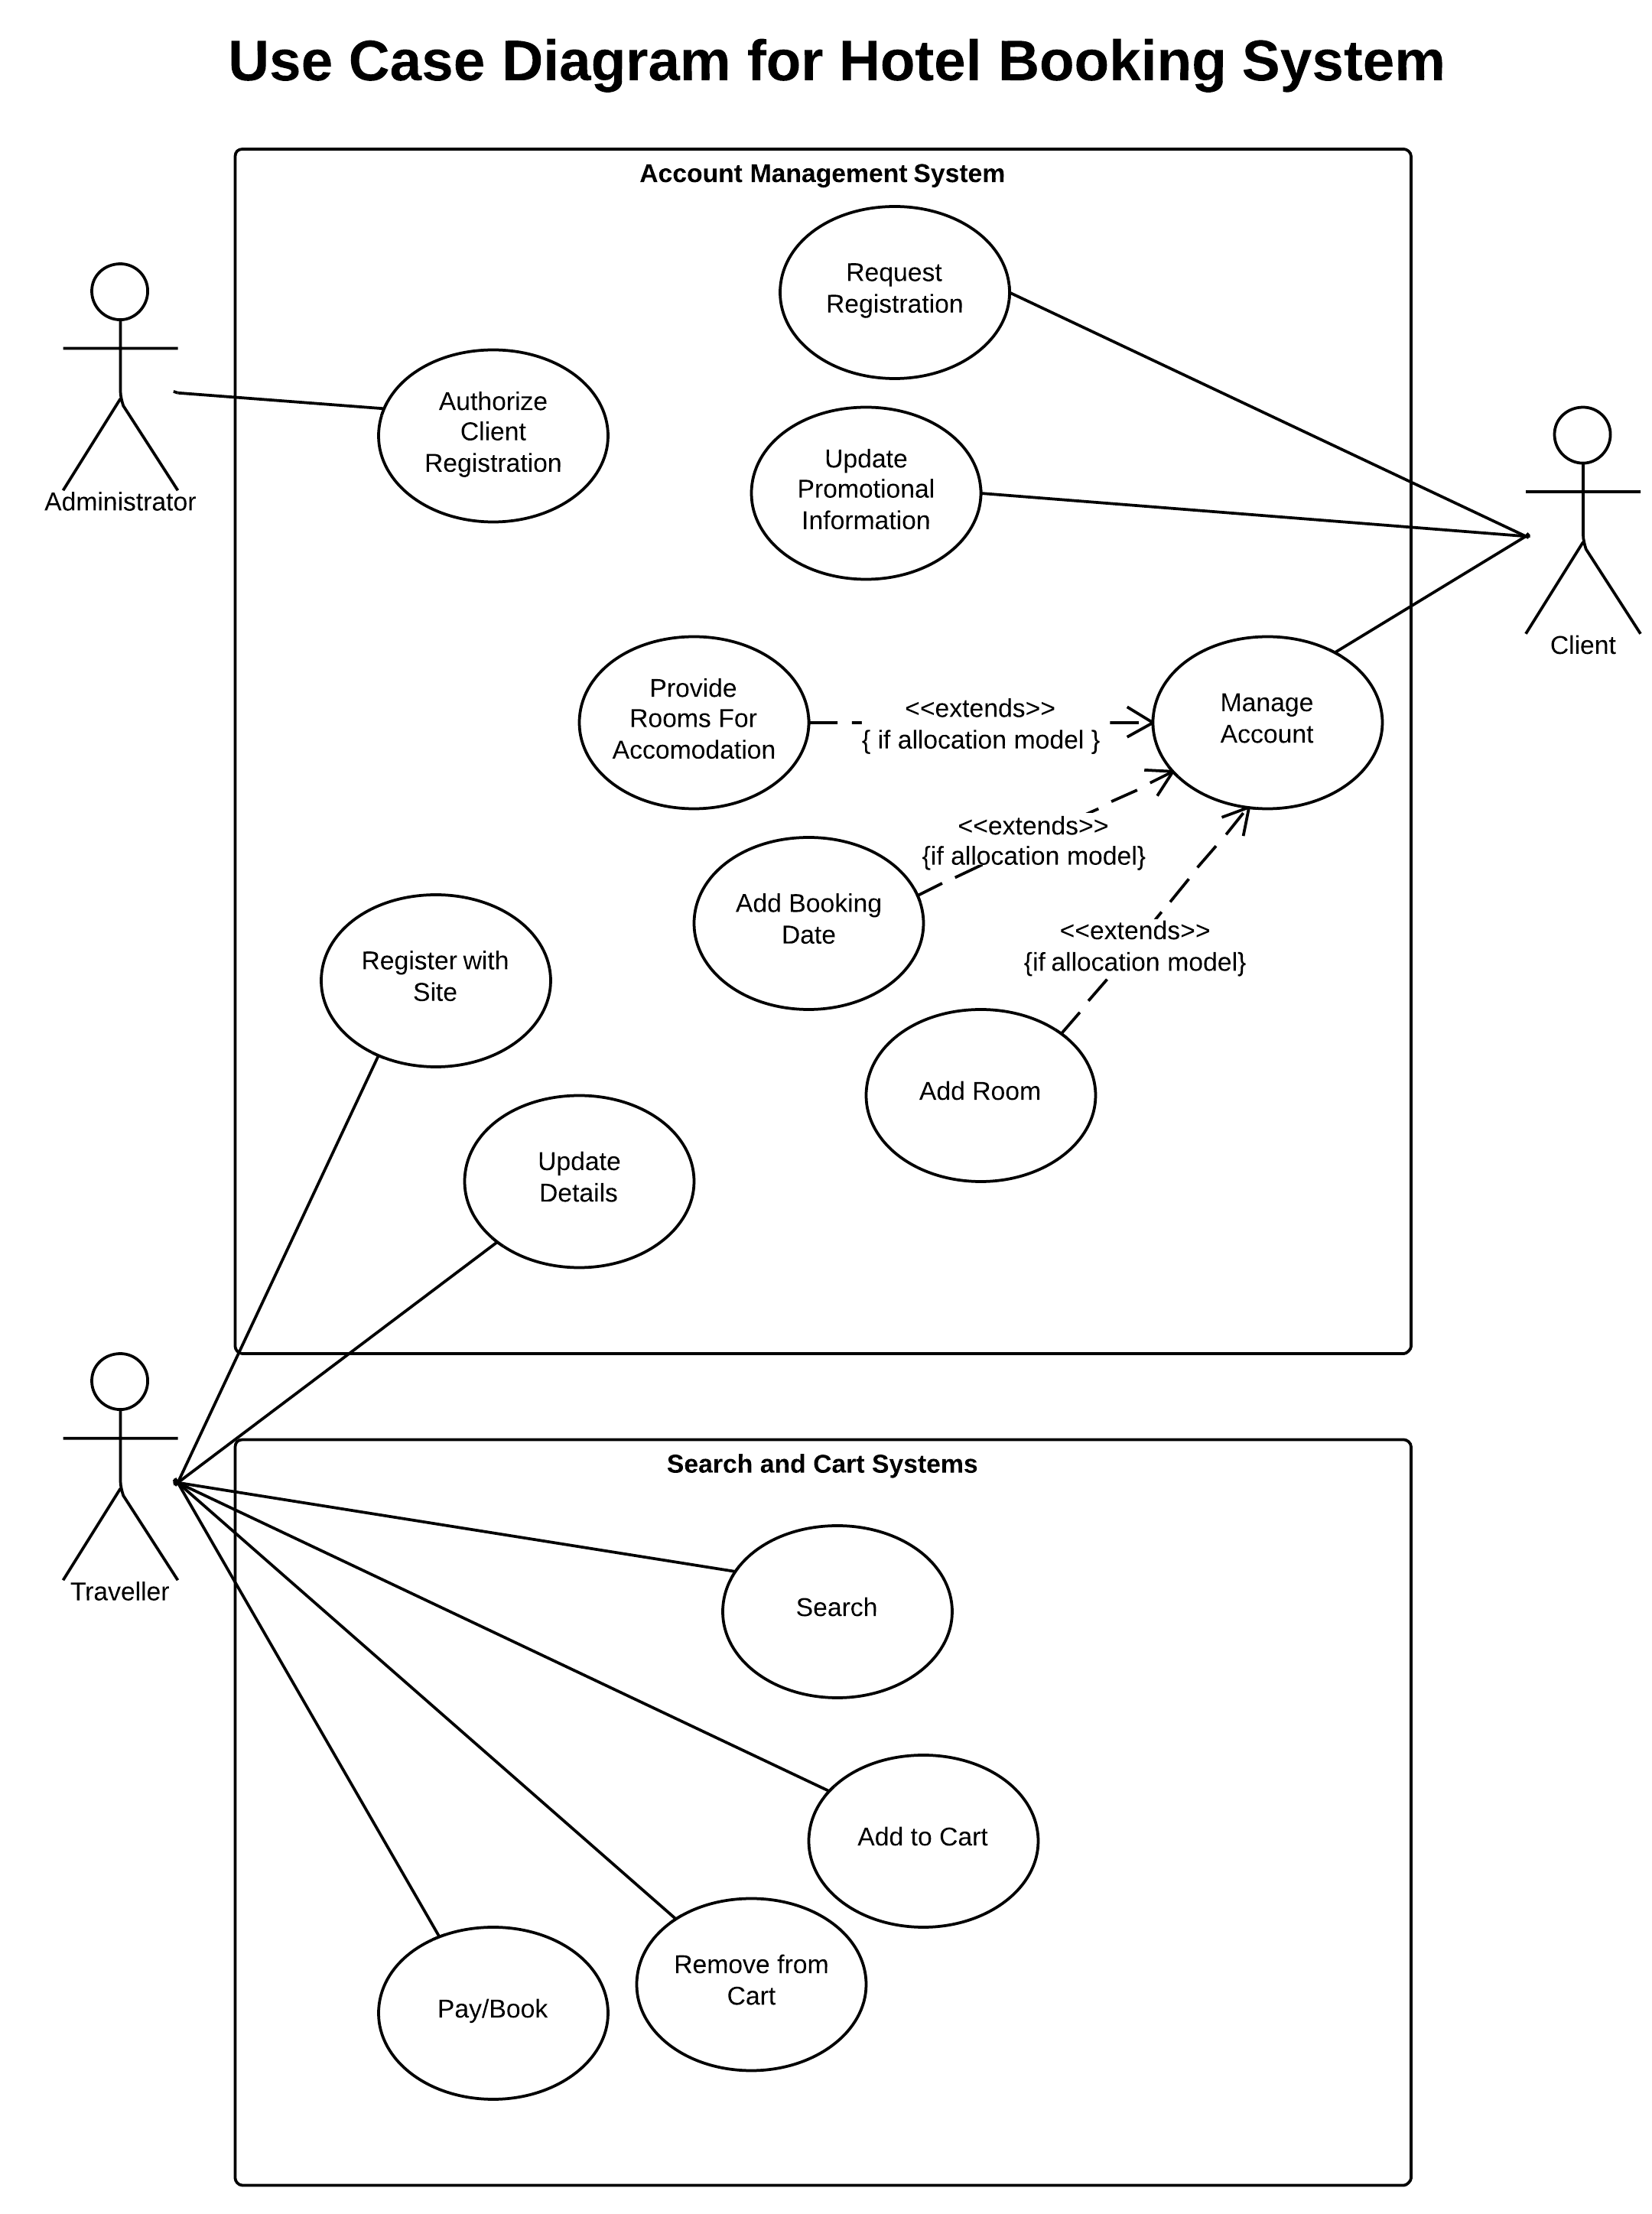
\includegraphics[width=1\textwidth]{img/UseCase.png}
\caption{Use Case diagram for the Hotel Site. Inc. all major actors.}
\label{fig:use-case}
\end{figure}

In figure \ref{fig:use-case}, the tasks each user can perform have been split into two sections. One outlining tasks to do with the management of a users account, and one to do with the actions of find and booking a hotel.

The major tasks a client can perform within the system are to request registration, update promotional information and manage their account. A client cannot directly register with the system. They must first make a request for registration which will later we authorised or declined by a system administrator. It is during this action that the client would be expected to provide details of which type of membership they require (e.g. allocation or referral model).

Updating promotional information fairly self explanatory. Clients will have the ability to change the description about their site that is displayed to travellers on the front end of the site.

Management of a client's account is a fairly broad task that encapsulates how clients can update the information about their site depending of the type of account they are given. If they are registered with a referral account, booking request details will be send to them via an automated email from the site. It is then the clients responsibility to respond to these requests. However, if the Client has a allocation type account, they will be able to update the number of rooms they have listed on the site, along with the dates which each of the rooms is booked for.

Travellers can perform tasks in both areas of the site. They have the ability to register with the site (no authorisation required) and can update their personal details stored with the site such as their card number and billing address.

They can also perform a variety of actions in relation to the search and cart systems such as search for a hotel based on a given criteria, adding/removing items to there cart and paying for the items in the cart when ready.

\subsection{Data Flow Diagram}
The next step in task analysis was to plan how data could possible flow between  actors, system tasks and data stores. I have provided the following data flow diagram to show how data might flow between the users and the tasks being performed by the booking site.

\begin{landscape}
\begin{figure}[H]
\centering
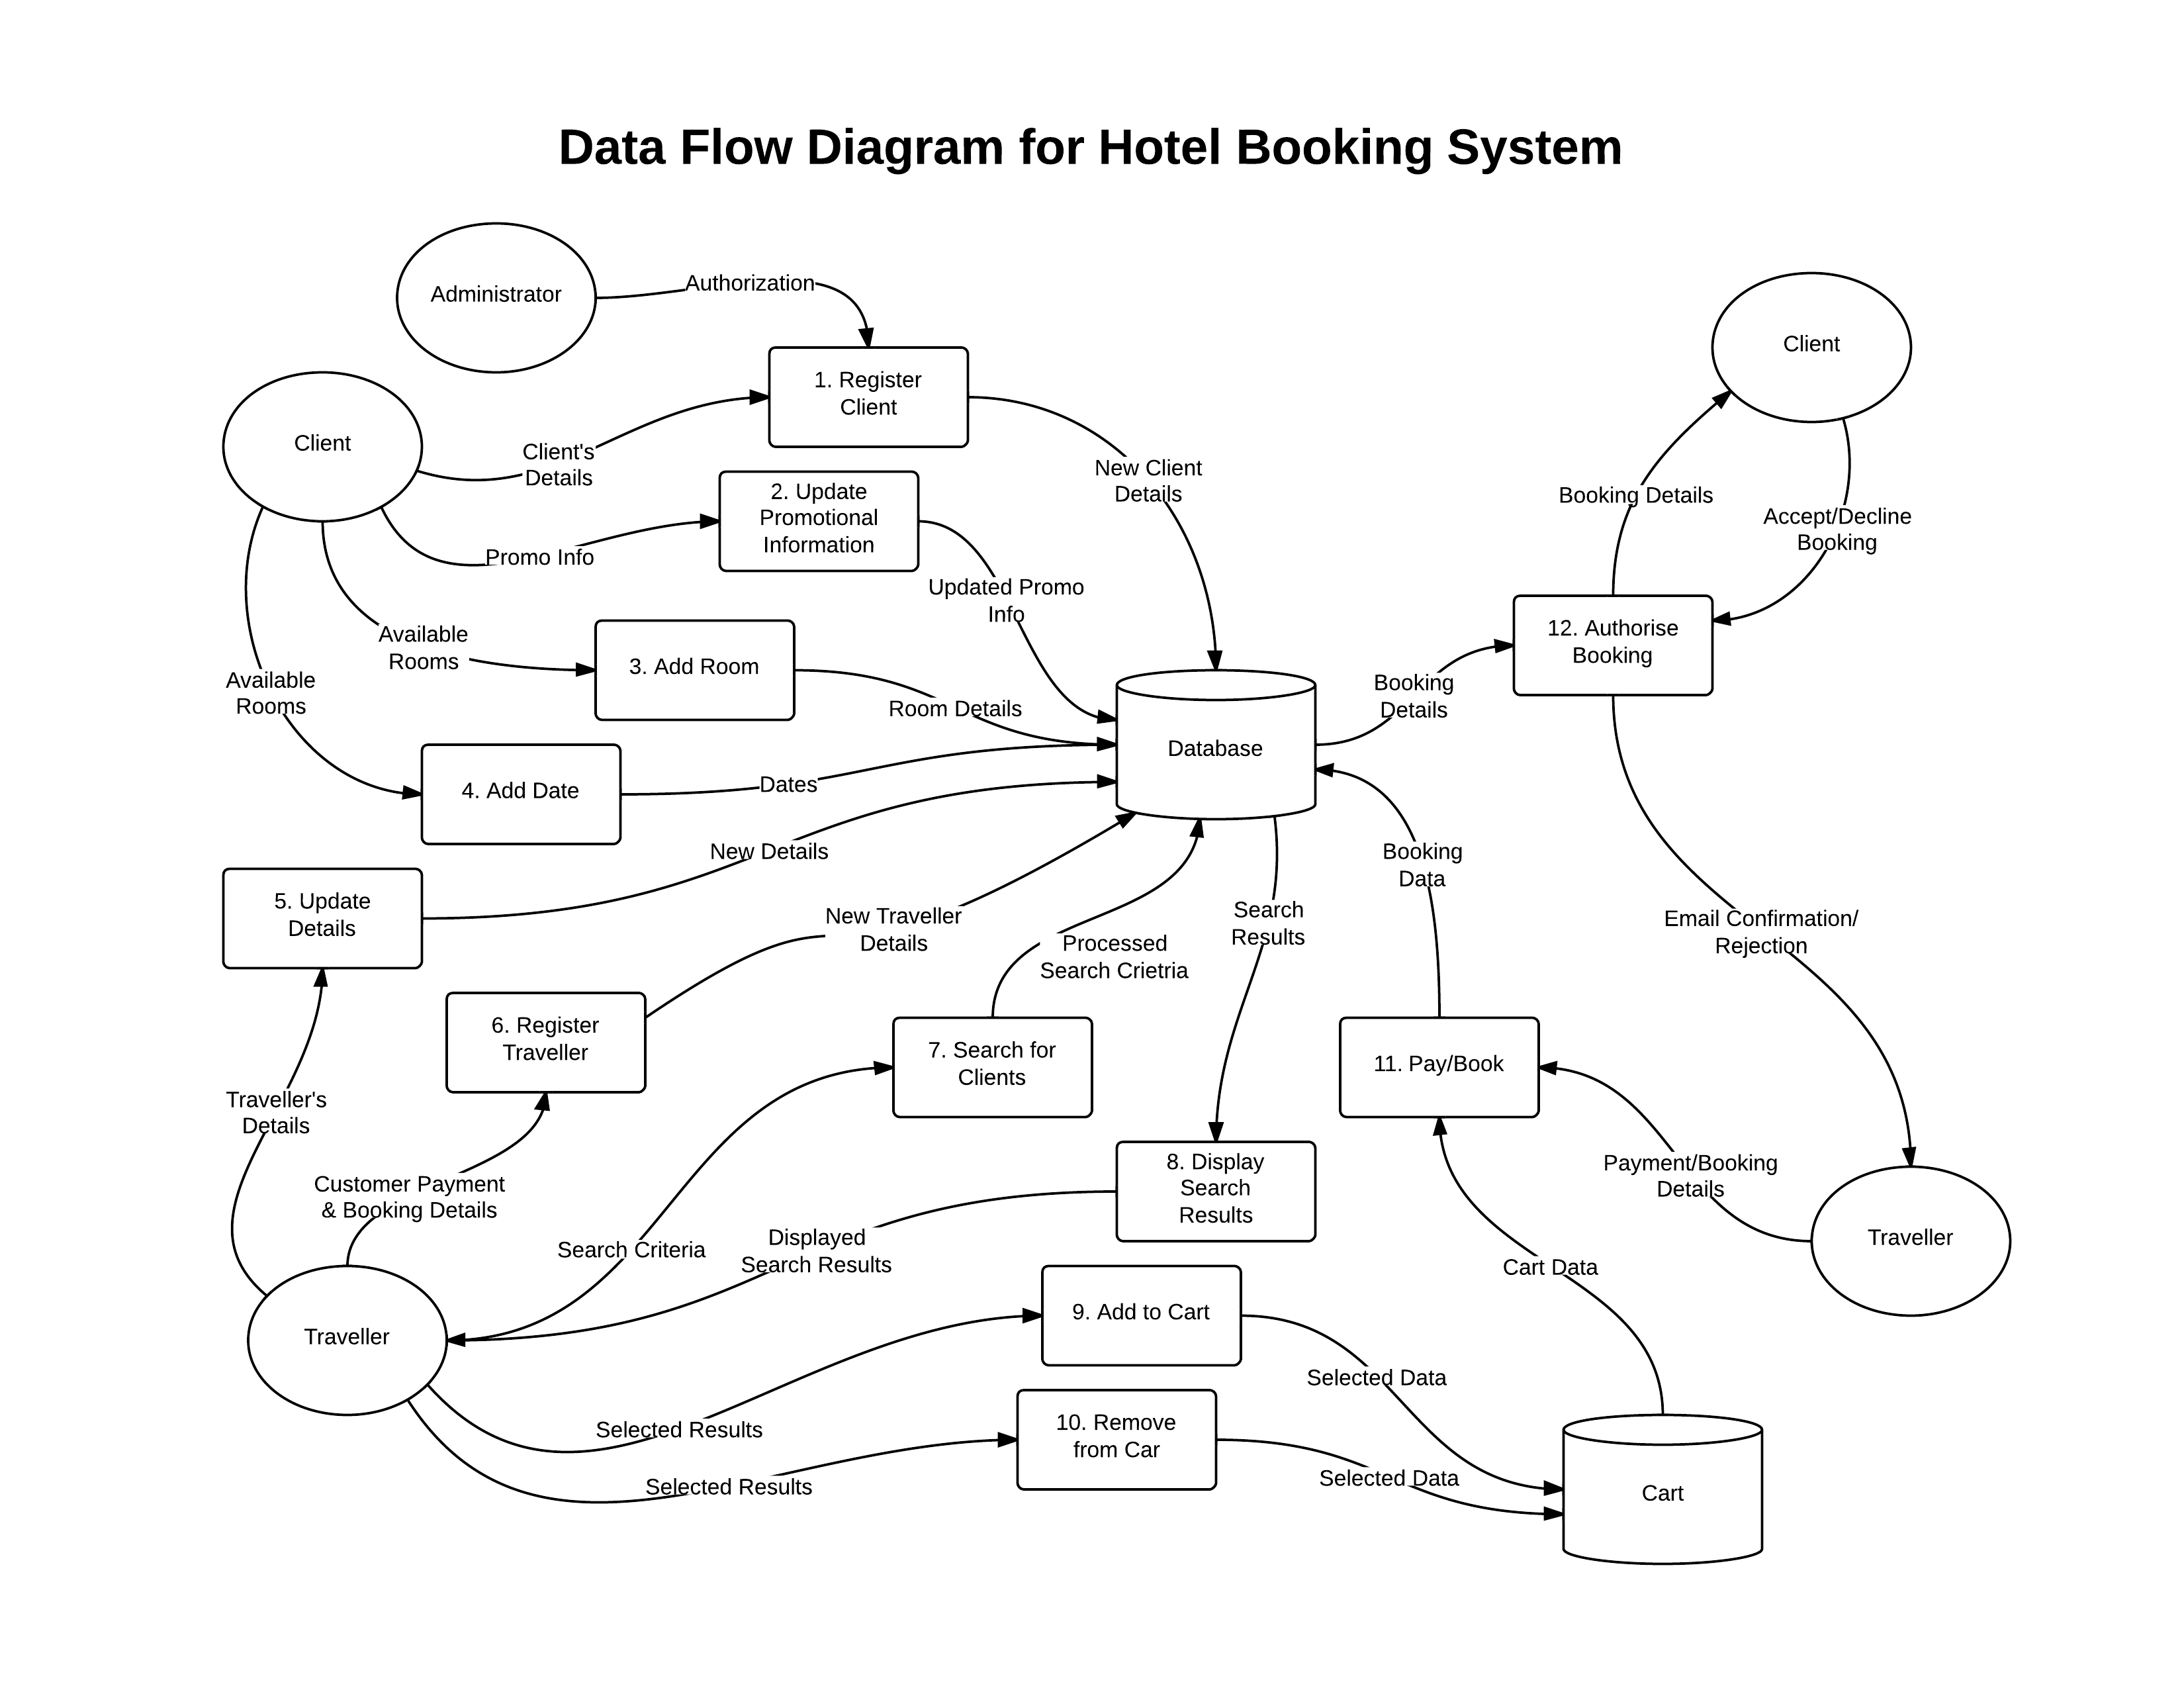
\includegraphics[angle=0, width=1\textwidth]{img/dataflow.png}
\caption{Data flow diagram for the Hotel Booking site.}
\label{fig:data-flow}
\end{figure}
\end{landscape}

Each of the major tasks identified in the use case analysis is shown, along with a bit more detail. Note that this diagram shows the flow of data for both the allocation and referral models as there are only a couple of differences between the two models. If a client is using the allocation model, The authorise booking stage would not be present as the booking would be completed automatically by the Hotel Site system and would therefore be unnecessary. Likewise, the ability for a client to add a room and add a booking date would not be present if the Client is assigned to the referral model.

Note that in this diagram I have visualised the cart as being a separate data store from the database. In an actual implementation, they would mostly likely be part of the same relational database model. However, I have decided to logically separate them here for clarity.

\subsection{State Transition Diagrams}
The final step in task analysis was to identify on a low level how the user can move between states in the system. For this section I provide a collection of state transition diagrams. These help to illustrate how users can move through a system to carry out desired tasks. The states shown also help to point out good possible starting points for the page designs outlined in the next section.

\begin{figure}[H]
\centering
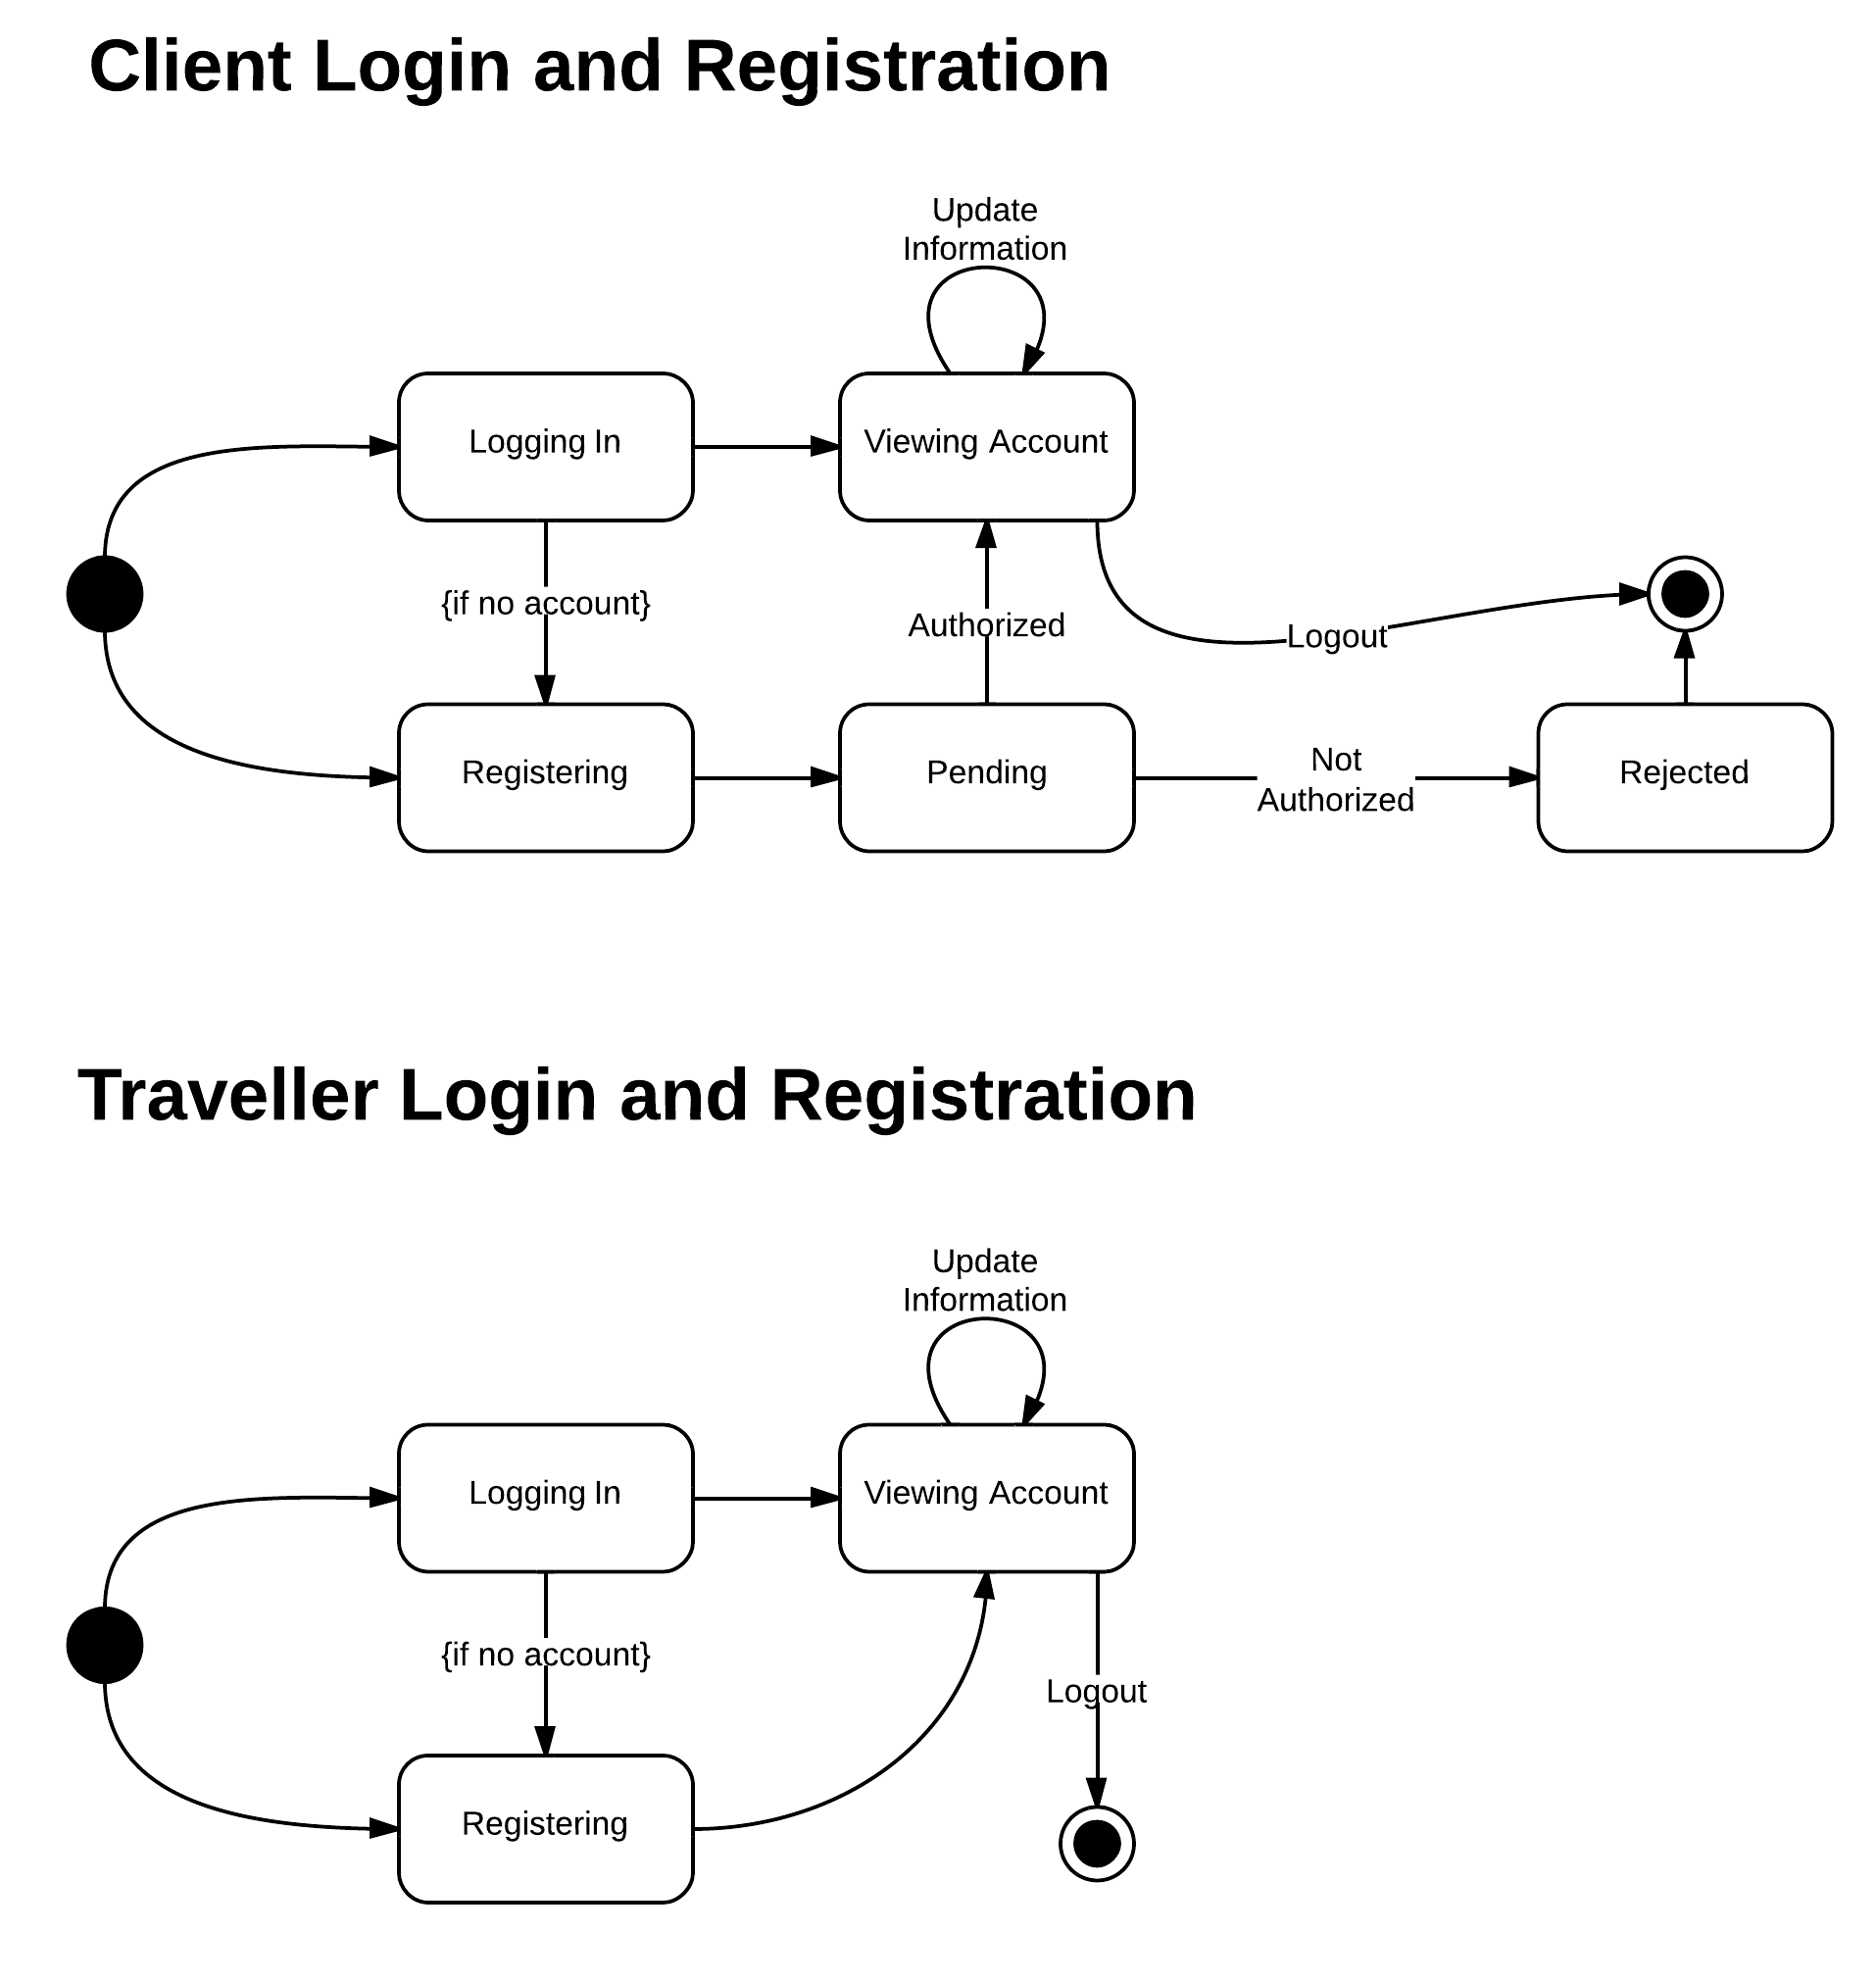
\includegraphics[width=0.7\textwidth]{img/state_diagrams/StateDiagramUserAuth.png}
\caption{State Transition diagrams for both Client and Traveller Login and Registration}
\label{fig:state-user-auth}
\end{figure}

Figure \ref{fig:state-user-auth} shows a comparison between the way that Clients and Travellers sign up for an account with the site and login for the site. In my design, it is planned that if a Client or Traveller attempts to perform an action that requires them to be logged in (such as viewing their account overview) and they have not yet logged in, they will be redirected automatically to the appropriate login page. Also note that Travellers will be required to register for an account or login before they can purchase the items stored in their cart.

Traveller login and registration is a fairly straight forward process. If a Traveller can login they go directly to the view account page. If they do not have an account yet, they can move to the registration page where they can get an account. They will then be diverted to the login page where they can perform further tasks. In the actual implementation, if the Traveller is asked to login/register during the process of buying the items in the cart, they will the not be sent to the account overview page, but redirected back into the buying process.

The Client login and registration process is very similar, but incorporates an extra step in the registration process. Because Client accounts need to be authorised by an administrator before Clients can use the management features, when a client registers they are moved into the pending state until their request for an account is either accepted or declined. Once it is accepted they can then proceed to use account management features.

\begin{figure}[H]
\centering
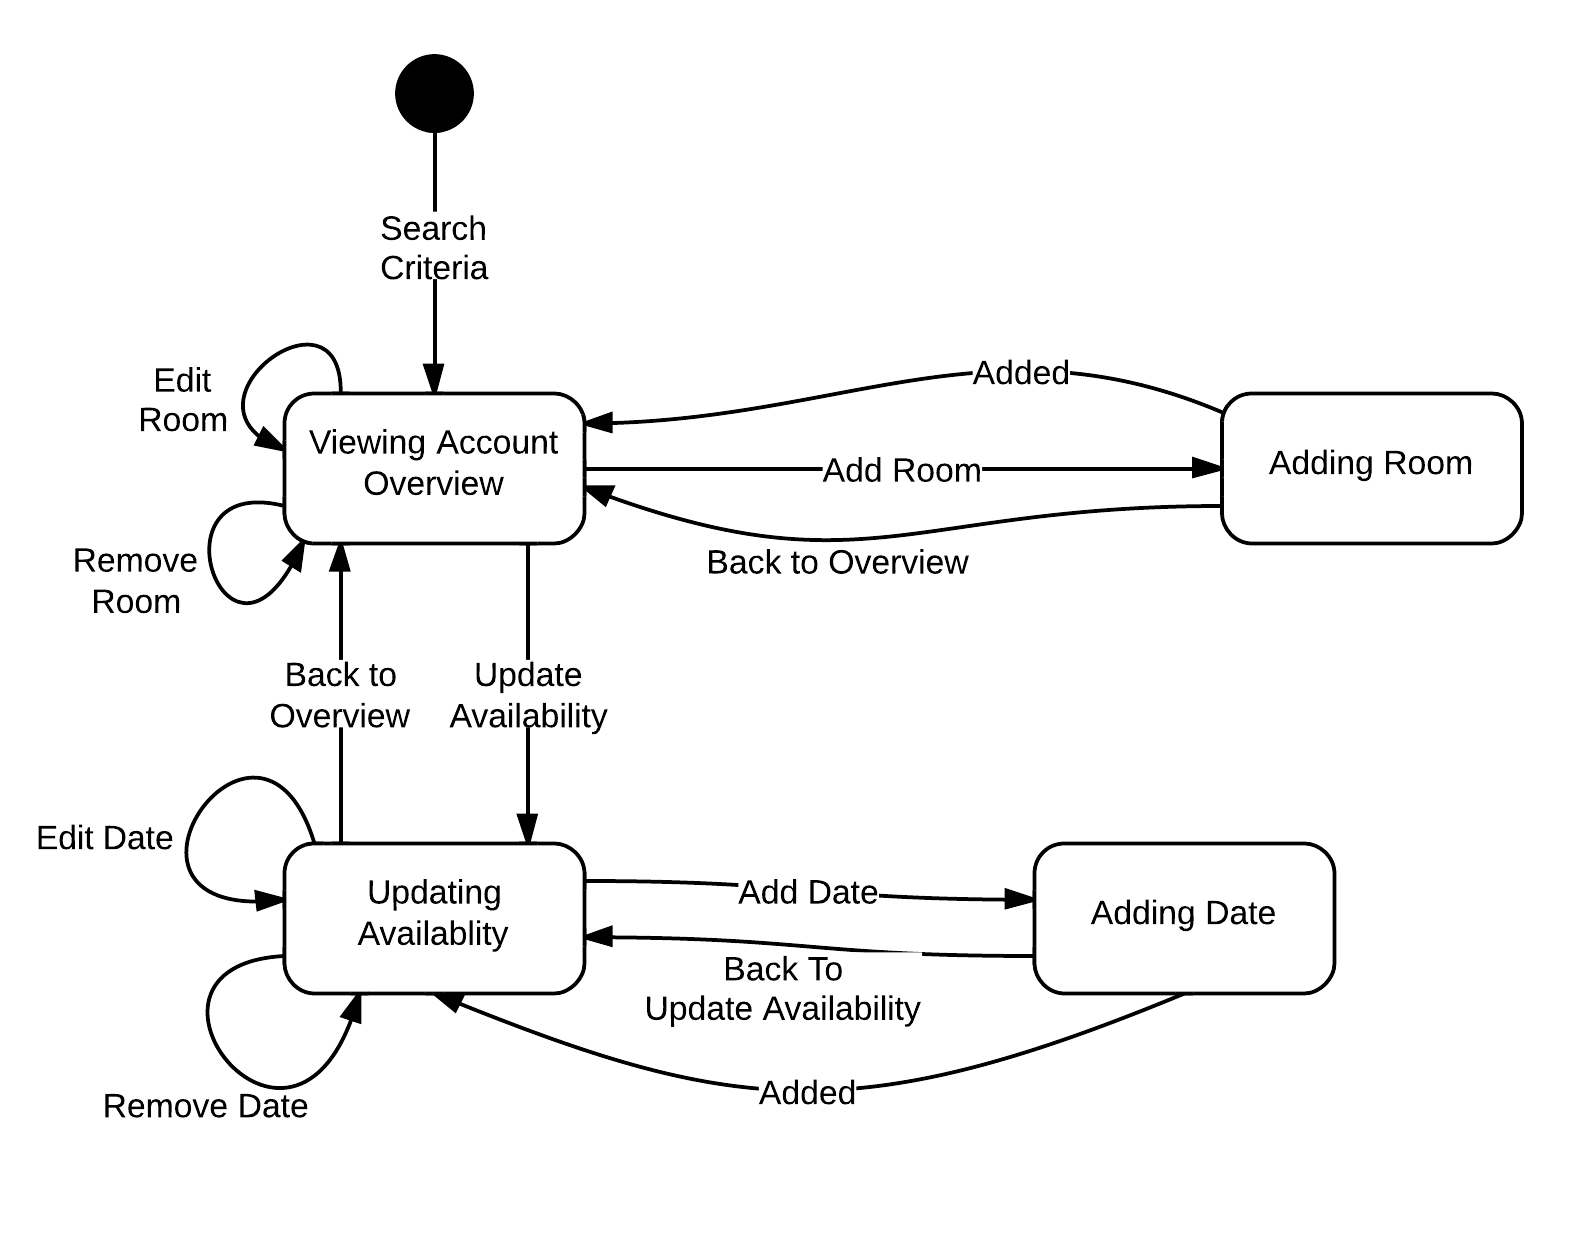
\includegraphics[width=0.7\textwidth]{img/state_diagrams/StateTransitionClientManagement.png}
\caption{State Transition diagram for Client account management}
\label{fig:state-client-manage}
\end{figure}

The next state transition diagram show in figure \ref{fig:state-client-manage} shows how Clients can moved between states of editing details about their account if they are using the allocation model. This state transition diagram is not applicable if the Client is using the referral model. In that case, the only action they are able to perform is the to update their promotional information.

This diagram shows the options a Client has to manage their account in greater detail. Here you can see that they have options to add, edit and remove a room and a booking date associated with a room. Transitions that state back to overview/update availability imply that not change was made to the system in the preceding state.

Each of the states in this diagram ultimately represents a page on the site and correlates to tasks that user might want to perform in this state. Note how editing and removing information does not require a change in state this is because each of the items will displayed in a form, so can be edited directly. In the real system edit and remove operations would mostly likely use AJAX or a simple page refresh to update the users interface after the operation has been carried out.

However, operations that require the user to add new information into the system require a change of state. This is because addition operations will require more information that from the user than an edit or remove operation and I therefore felt that it would be more clear what information was required if the user was moved to another state to breakdown the number of options a Client can choose in any single state. In any single state during Client management, the Client is not presented with more than five possible operations at once.

\begin{figure}[H]
\centering
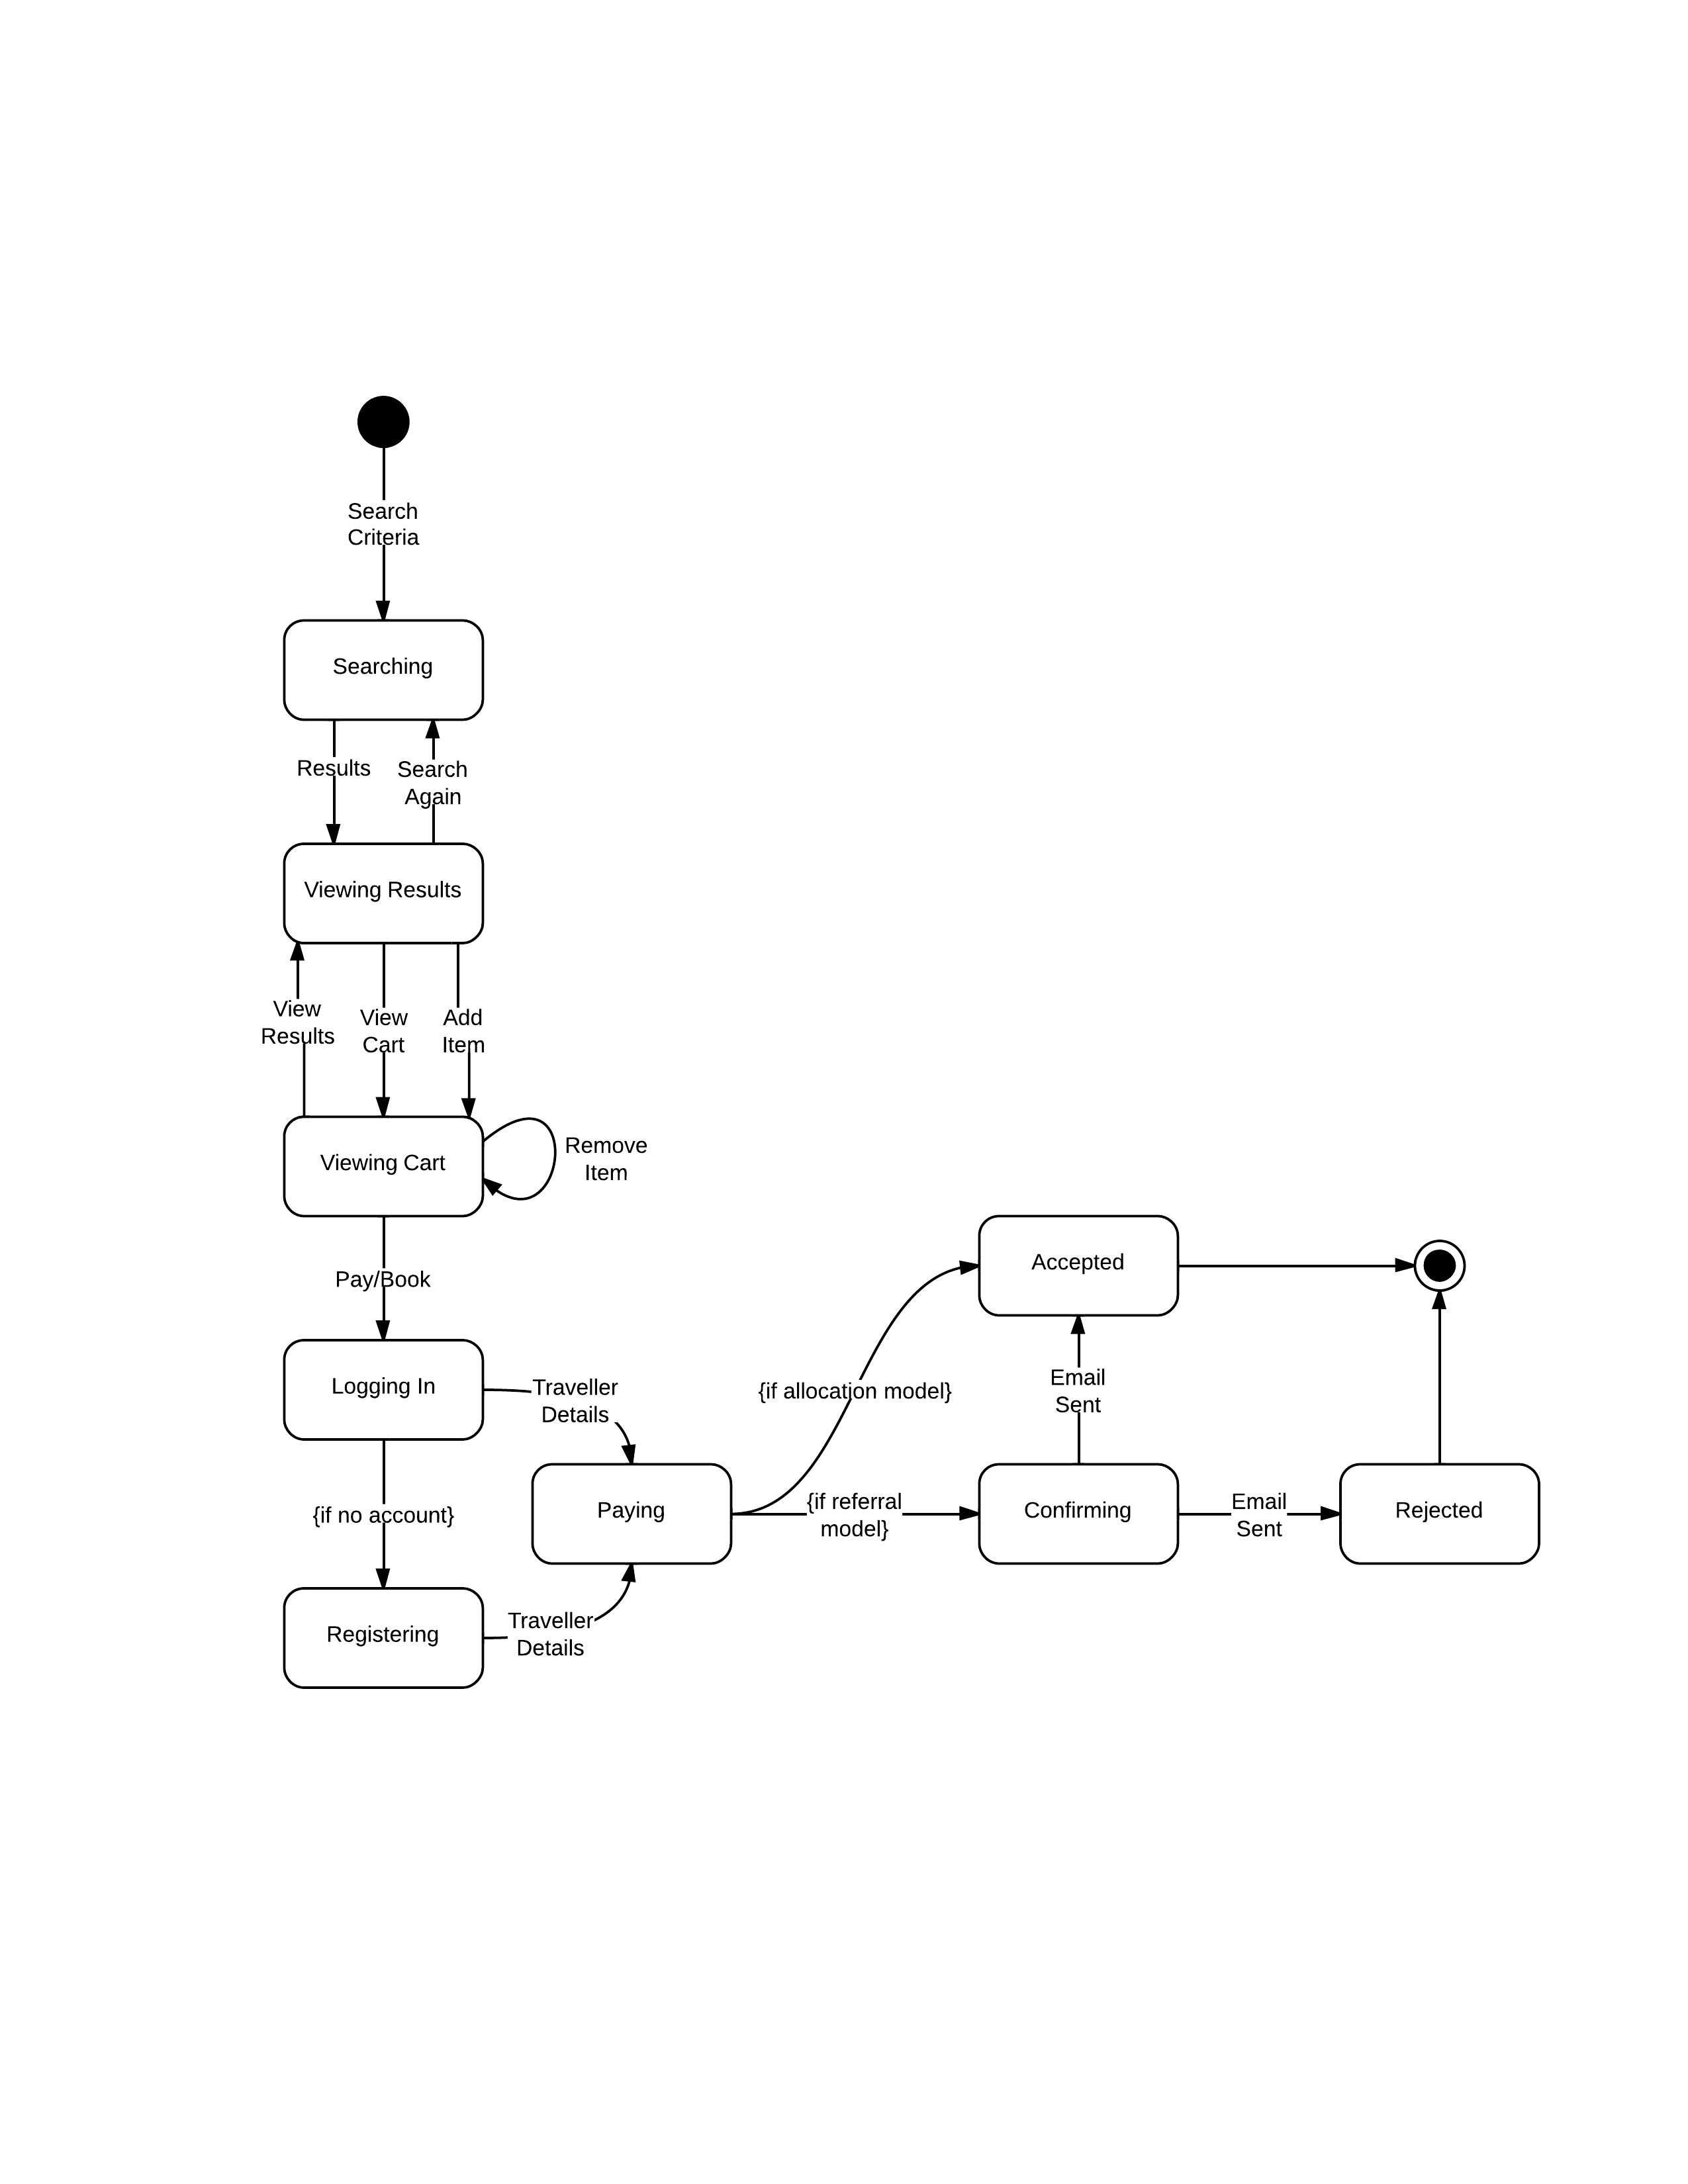
\includegraphics[width=0.7\textwidth]{img/state_diagrams/StateTransitionDiagramUserPayement.png}
\caption{State Transition diagram for Traveller Search, Booking and Payment}
\label{fig:state-traveller-book}
\end{figure}

The final state transition diagram shown in figure \ref{fig:state-traveller-book} shows how a Traveller moves through states in the booking process from initially starting a search through to paying and booking their selected options. Their are several key points in the diagram worth point out. Firstly, note that a Traveller and move freely between searching, viewing results and viewing their cart until they are ready to pay and book. Once they have started down the payment/booking path, they a follow a more linear flow through the system. This was designed to try an emulate a "checkout" feeling of clear operation that need to be performed once the user is comfortable with their choices.

I have also incorporated in the diagram the option for either logging in or going to registering state if the Traveller does bot yet have an account. Note that unlike in figure \ref{fig:state-user-auth} they are not redirected to their account overview, but are returned back into the payment/booking "flow".

Finally, depending on the type of booking model the Hotel is registered with, the Travellers booking will either be automatically accepted (as with the allocation model) or  (in the case of the referral model) the Traveller will move into the "confirming" stage where they will wait until there booking is either confirmed or declined by hotel itself.

\section{Interaction Design}
The next section of this document is concerned with the interaction design for the  Hotel Booking website. This includes a large set of high level wire frame designs for the major pages in the site. In short, this section defines the general structure of the user interface for the website, without real regard for the site's internal operation.



\section{Prototype}


\section{Discussion}
\end{document}